%#
%# Lab study
%# https://github.com/IIS-Lab/ShibatoM/wiki/Analysis-of-lab-study をまとめる.
%############################

\chapter{RealCodeが出題する演習問題の分類評価}
\label{section:lab-study}
\graphicspath{{Chapters_evaluation/Figs/}}


\ref{section:ta_evaluation},\ref{section:interview-study}章にて述べたRealCodeの評価実験により,イシューをプログラミング演習問題へと転用することで,既存の学習環境にはない独自の演習問題を提供できることが明らかとなった.
しかし,RealCodeの演習問題からどのような内容(例えば文法やアルゴリズム)を学習できるのかは明らかとなっていない.
そこで,RealCodeの演習問題から学習可能な内容を理解するために,著者によるRealCodeの演習問題の分類評価を行った.


\section{実験方法}

現在のRealCodeのプロトタイプに存在する116件のPythonの演習問題に対し,図\ref{fig:lab-study}に示す分類評価用のインターフェースから,著者は以下の質問に回答した.

\begin{itemize}
  \item[Q1.] This is a good exercise to you. (1: Disagree -- 3: Agree)
  \item[Q2.] What did you learn from this exercise?
  \begin{itemize}
  	  \item 文法
   	  \item アルゴリズム
      \item ライブラリやAPIの使い方
      \item 自分が経験した・見たことのあるバグの解決方法
      \item ソフトウェアのテスト
      \item デザイン
      \item ウェブ
      \item データベース
      \item 例外処理
      \item メンテナンス
      \item その他学んだこと(記述式)
  \end{itemize}
\end{itemize}

\begin{figure}[H]
 \centering
  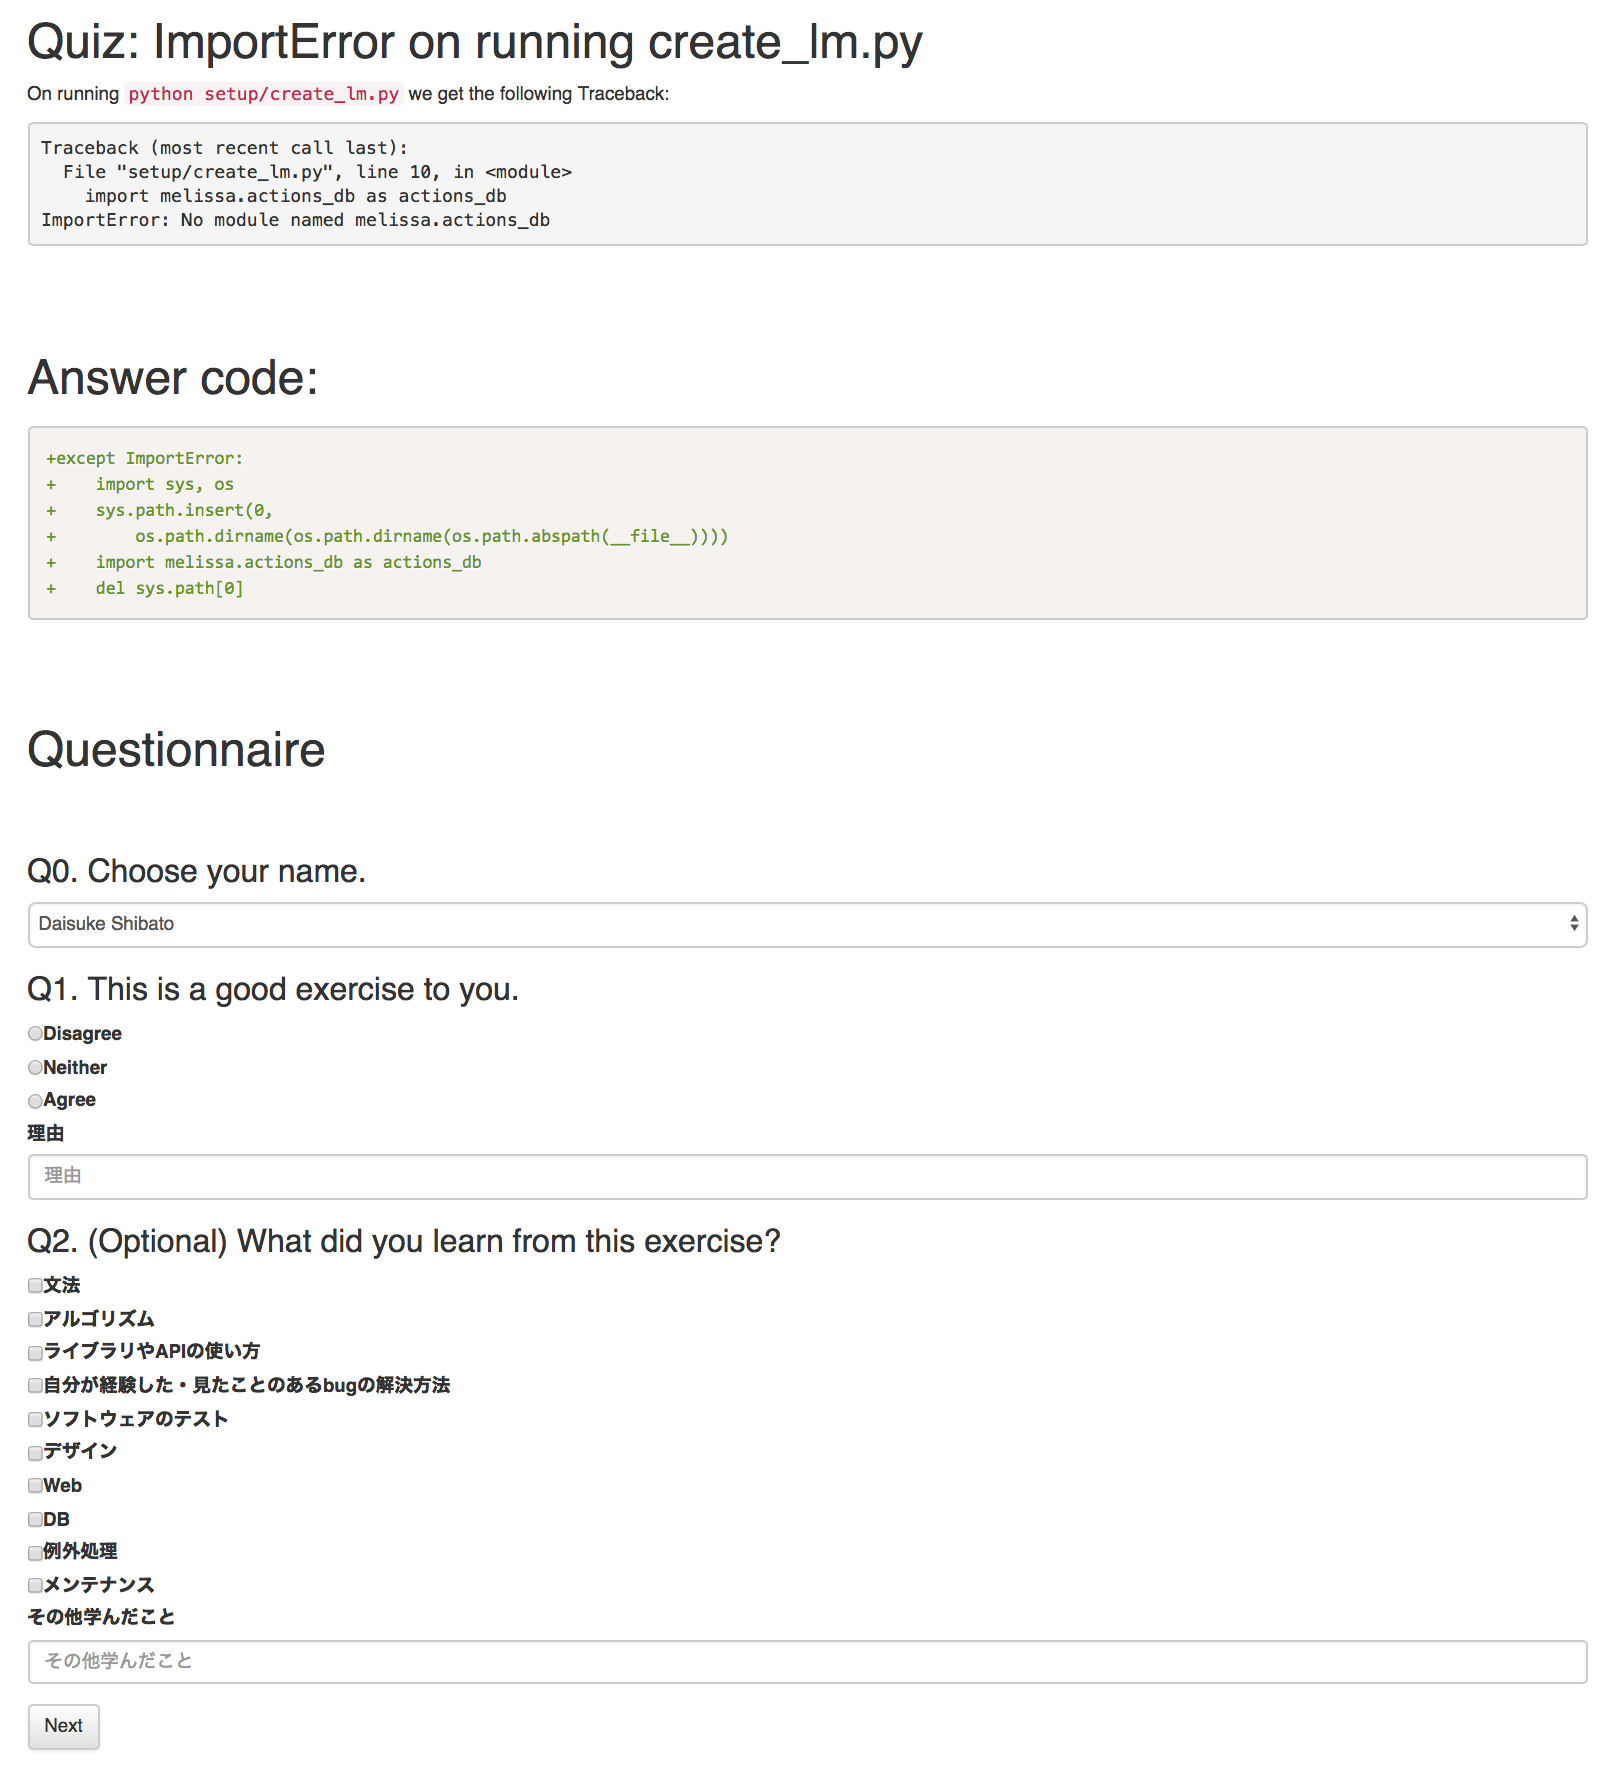
\includegraphics[width=1.0\columnwidth]{20181218-lab-study-interface-all.png}
  \caption{RealCodeが出題する演習問題の分類評価にて用いたインターフェース.}
  \label{fig:lab-study}
\end{figure}

\section{実験結果と考察}

\begin{table}[b]
  \centering
  \caption{RealCodeが出題する演習問題の分類評価におけるQ2の結果.但し,母数はQ1に対し``Agree''と回答された48問の演習問題である.}
  \label{table:lab-study-q2-result}
  \begin{tabular}{ l | c } \Xhline{3\arrayrulewidth}
      分類 & 割合(\%) \\ \hline \hline
      例外処理 & 12.85 \\
      メンテナンス & 12.29  \\
      自分が経験した・見たことのあるバグの解決方法 & 9.50 \\
      ライブラリやAPIの使い方 & 6.70 \\
      アルゴリズム & 2.79 \\
      Web & 2.79 \\
      文法 & 1.12 \\  
      デザイン & 0.56 \\
      DB & 0.56 \\
      \Xhline{3\arrayrulewidth}
  \end{tabular}
\end{table}

Q1に対して,41.4\%の演習問題が``Agree'',18.1\%が``Neither'',40.5\%が``Disagree''として回答した.
また``Disagree''の理由として,1)コード変更がわかりづらい,2)リファクタリングのみが行われている,3)著書が知らなかったライブラリのAPIが多く使用されている,の3つの要因が多く挙げられた.

回答結果を確認した結果,コード変更がわかりづらい要因として,コード変更量が数行程度といった断片的なものであることや,既存の関数の一部の変更といった局所的なものであることが明らかとなった.
また,使用されている変数の多くがコード変更の外で宣言されている場合も,コード変更がわかりづらいと判断した.
これらのような演習問題をデータセットから除外する手法の一つとして,演習問題のコード変更と全体のソースコードの構文解析を行い,外部変数の使用割合や文法的コード変更の分類を特徴量として決定木に与えることが考えられる.
しかし,現在のRealCodeのプロトタイプは様々なプログラミング言語に対応するために意図的に構文解析を導入していない.
RealCodeの演習問題において頻繁に使用されているプログラミング言語の構文解析を実装することで,RealCode上の演習問題数を保ちながら,コード変更がわかりづらい演習問題を除外できると考える.

また,リファクタリングのみが行われている演習問題からはプログラミングに関する知識を得ることができないと判断した.
なぜなら,リファクタリングのコード変更は変数名やインデントの変更などのみから構成されているためである.
コード変更がリファクタリングであるかどうかを判定するためには,構文解析を使用した手法と,コード変更の繰り返しを検出する手法が考えられる.
構文解析を用いてコード変更が構造的に変更されているかどうかを判定することで,一般的に構造的には変更しないリファクタリングを検出できると考えられる.
また,コード変更内に繰り返し発生する変更パターンを検出できた場合も,リファクタリングであると判断できる.
後者は構文解析を用いることなく実装できるため,様々なプログラミング言語に対応しながら実装することができる可能性がある.

また,著者が知らなかったライブラリのAPIが多く使用されている演習問題では,そもそもコード変更を理解することができなかったため``Disagree''と回答した.
このような演習問題の多くが,デバッグツールやコンソールアプリといった,著者にとってあまり馴染みのないリポジトリから生成されていた.
ユーザのプログラミング経験や知識に応じて,演習問題の生成元であるリポジトリをあらかじめ選定できるようになれば,ユーザが知らないライブラリが多く使用された演習問題を除外できる可能性がある.

次に,Q2の回答結果を表\ref{table:lab-study-q2-result}に示す.
特に回答の割合の高かった例外処理,メンテナンス,自分が経験した・見たことのあるバグの解決方法,ライブラリやAPIの使い方の4つの分類について考察を行う.


\subsection{例外処理に関する演習問題}

例外処理に関して学ぶことができるとラベル付けされた演習問題には,文字コードのエンコードエラーやネットワークの接続エラーが発生した際の対応策に関するものが多く含まれていた.
例えば図\ref{fig:lab-study-eg-exception}に示す演習問題では,Pythonのtry,catch構文を用いて``Unicode Encode Error''という例外に対応している.
ソフトウェアを本番稼働させるためには,起こりうる例外を想定しあらかじめ対策しておくことが重要であるが,一般的なプログラミング演習問題ではあまり扱われていない~\cite{Piteira_Learning_Computer_Programming}.
RealCodeの例外処理に関する演習問題を通じて,ソフトウェアを本番稼働させた際に発生しうる例外とその対応策に関する知識を習得できる可能性がある.

\begin{figure}[H]
  \centering
  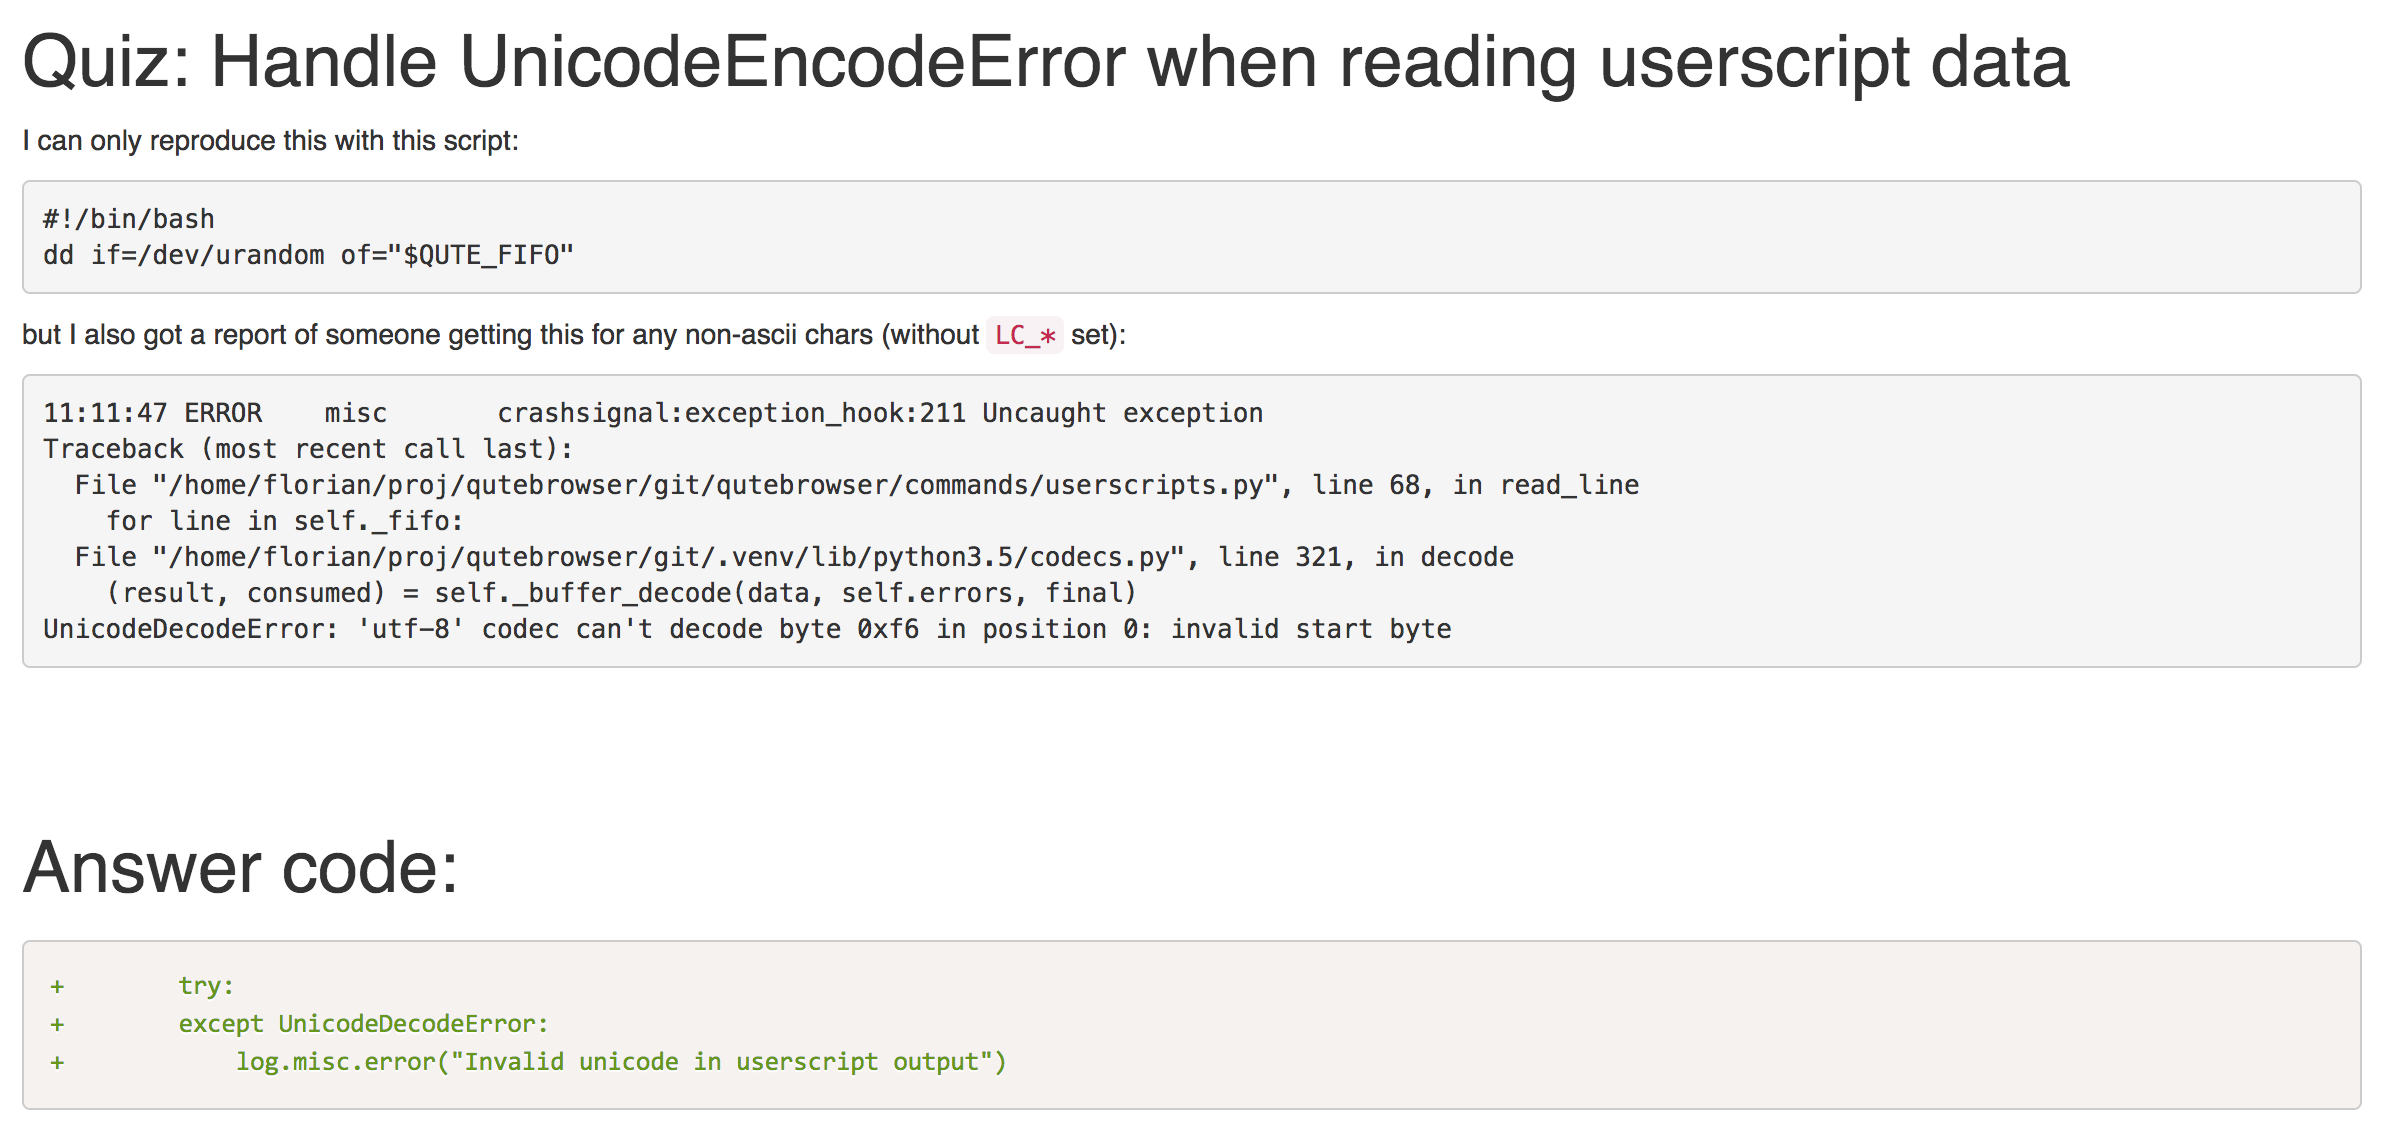
\includegraphics[width=1.0\columnwidth]{20190107-lab-study-exception-exercise2.png}
  \caption{例外処理に関する演習問題の例.``Unicode Encode Error''の例外に対して,Pythonのtry,catch構文を用いて対応している.}
  \label{fig:lab-study-eg-exception}
\end{figure}


\subsection{メンテナンスに関する演習問題}

本番稼働中のソフトウェアにて障害が発生した際に迅速に対応するためには,動作中のソフトウェアのログを取得しておくことが重要である~\cite{kernighan1999practice}.
図\ref{fig:lab-study-eg-maintenance}に示す演習問題の例では,動作しているソフトウェアのプロセス番号をログに追加するコード変更を行なっている.
プロセス番号があらかじめ分かっていれば,ソフトウェアの動作状況を監視できると同時に,障害発生時にも速やかな対応を行うことが可能となる.
RealCodeのメンテナンスに関する演習問題から,ソフトウェアの実装だけでなく,運用していく上での知識も学習できる可能性がある.

\begin{figure}[H]
\vspace{-0.05cm}
	\centering
  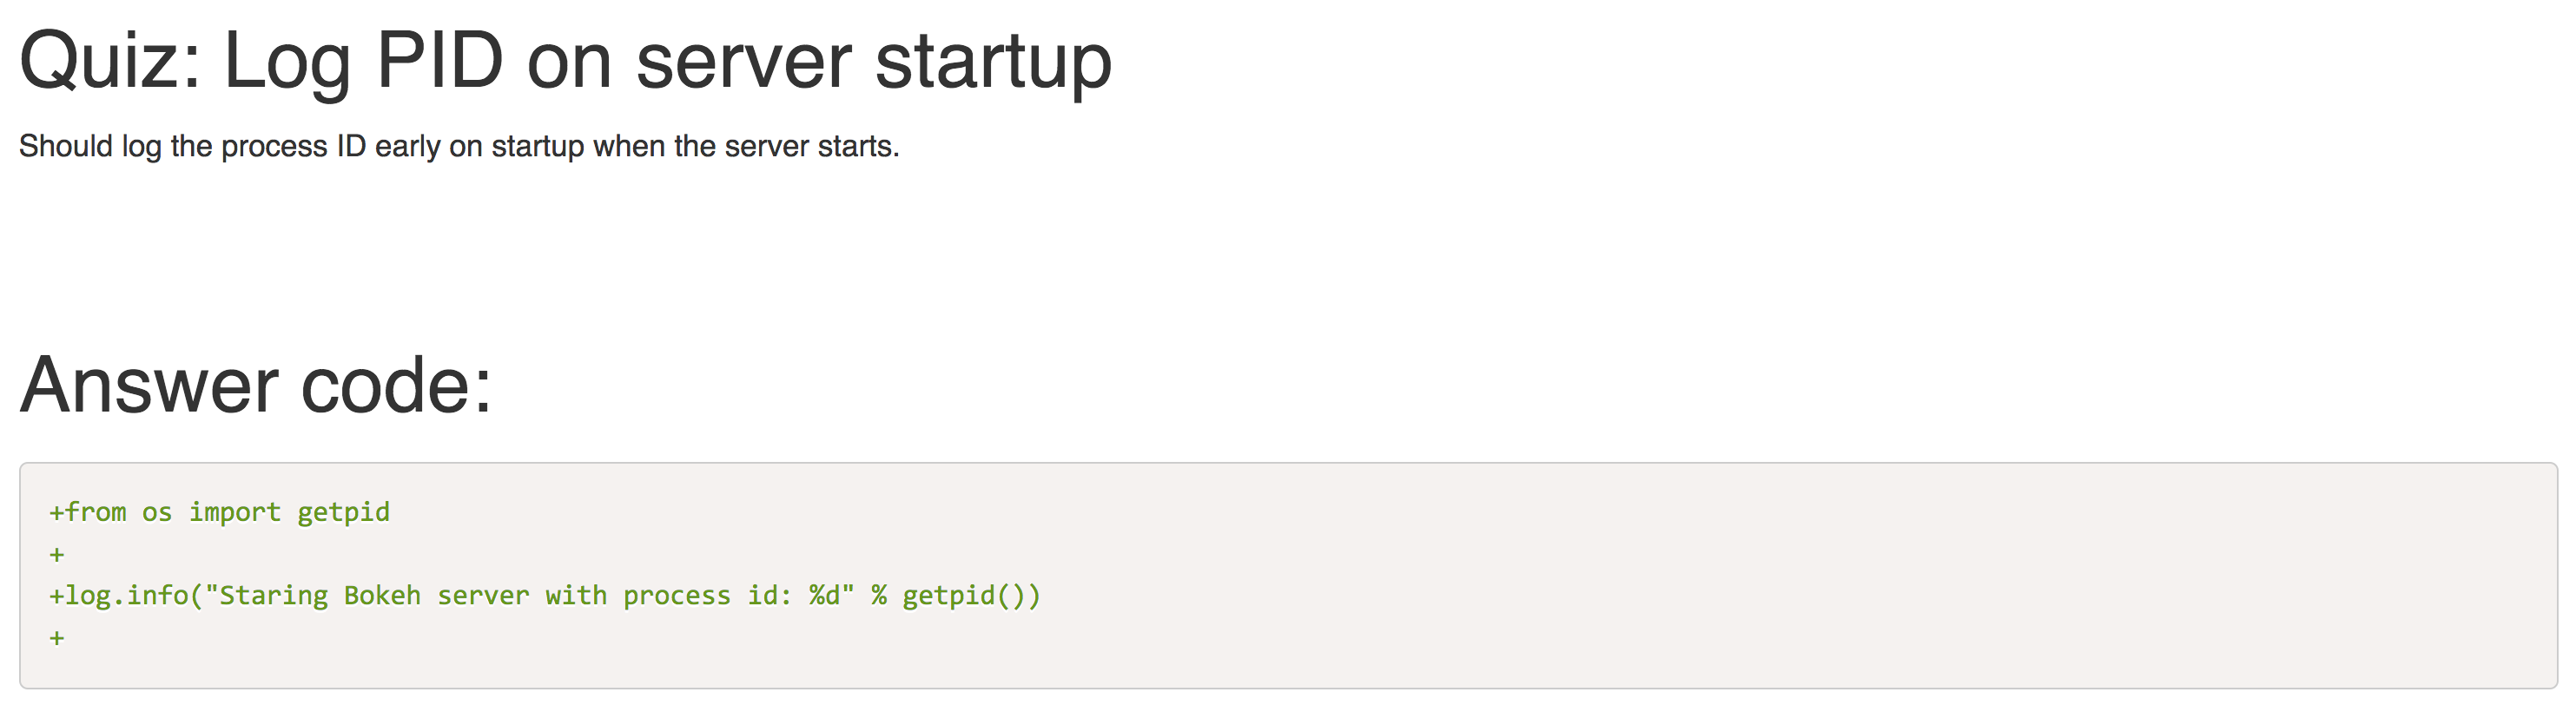
\includegraphics[width=0.95\columnwidth]{20190107-lab-study-maintenance-exercise.png}
  \vspace{-0.05cm}
  \caption{ソフトウェアのメンテナンスに関する演習問題の例.起動時にプロセス番号をログに出力している.}
  \label{fig:lab-study-eg-maintenance}
  \vspace{-0.35cm}
\end{figure}

\subsection{自分が経験した・見たことのあるバグの解決方法に関する演習問題}

RealCodeの演習問題はGitHubに実在するイシューとプルリクエストから生成されており,頻発するバグに関する演習問題が多く含まれている.
図\ref{fig:lab-study-eg-experience}に示す演習問題では,データベースの名前にピリオドは使用できないという,データベースを扱う際に頻発するバグを取り扱っている.
このようなプログラミングの基礎知識ではないが実装する上でよく発生する問題は一般的なプログラミング学習材料では扱われておらず,RealCode特有の演習問題であると言える.

\begin{figure}[H]
 \centering
 \vspace{-0.3cm}
 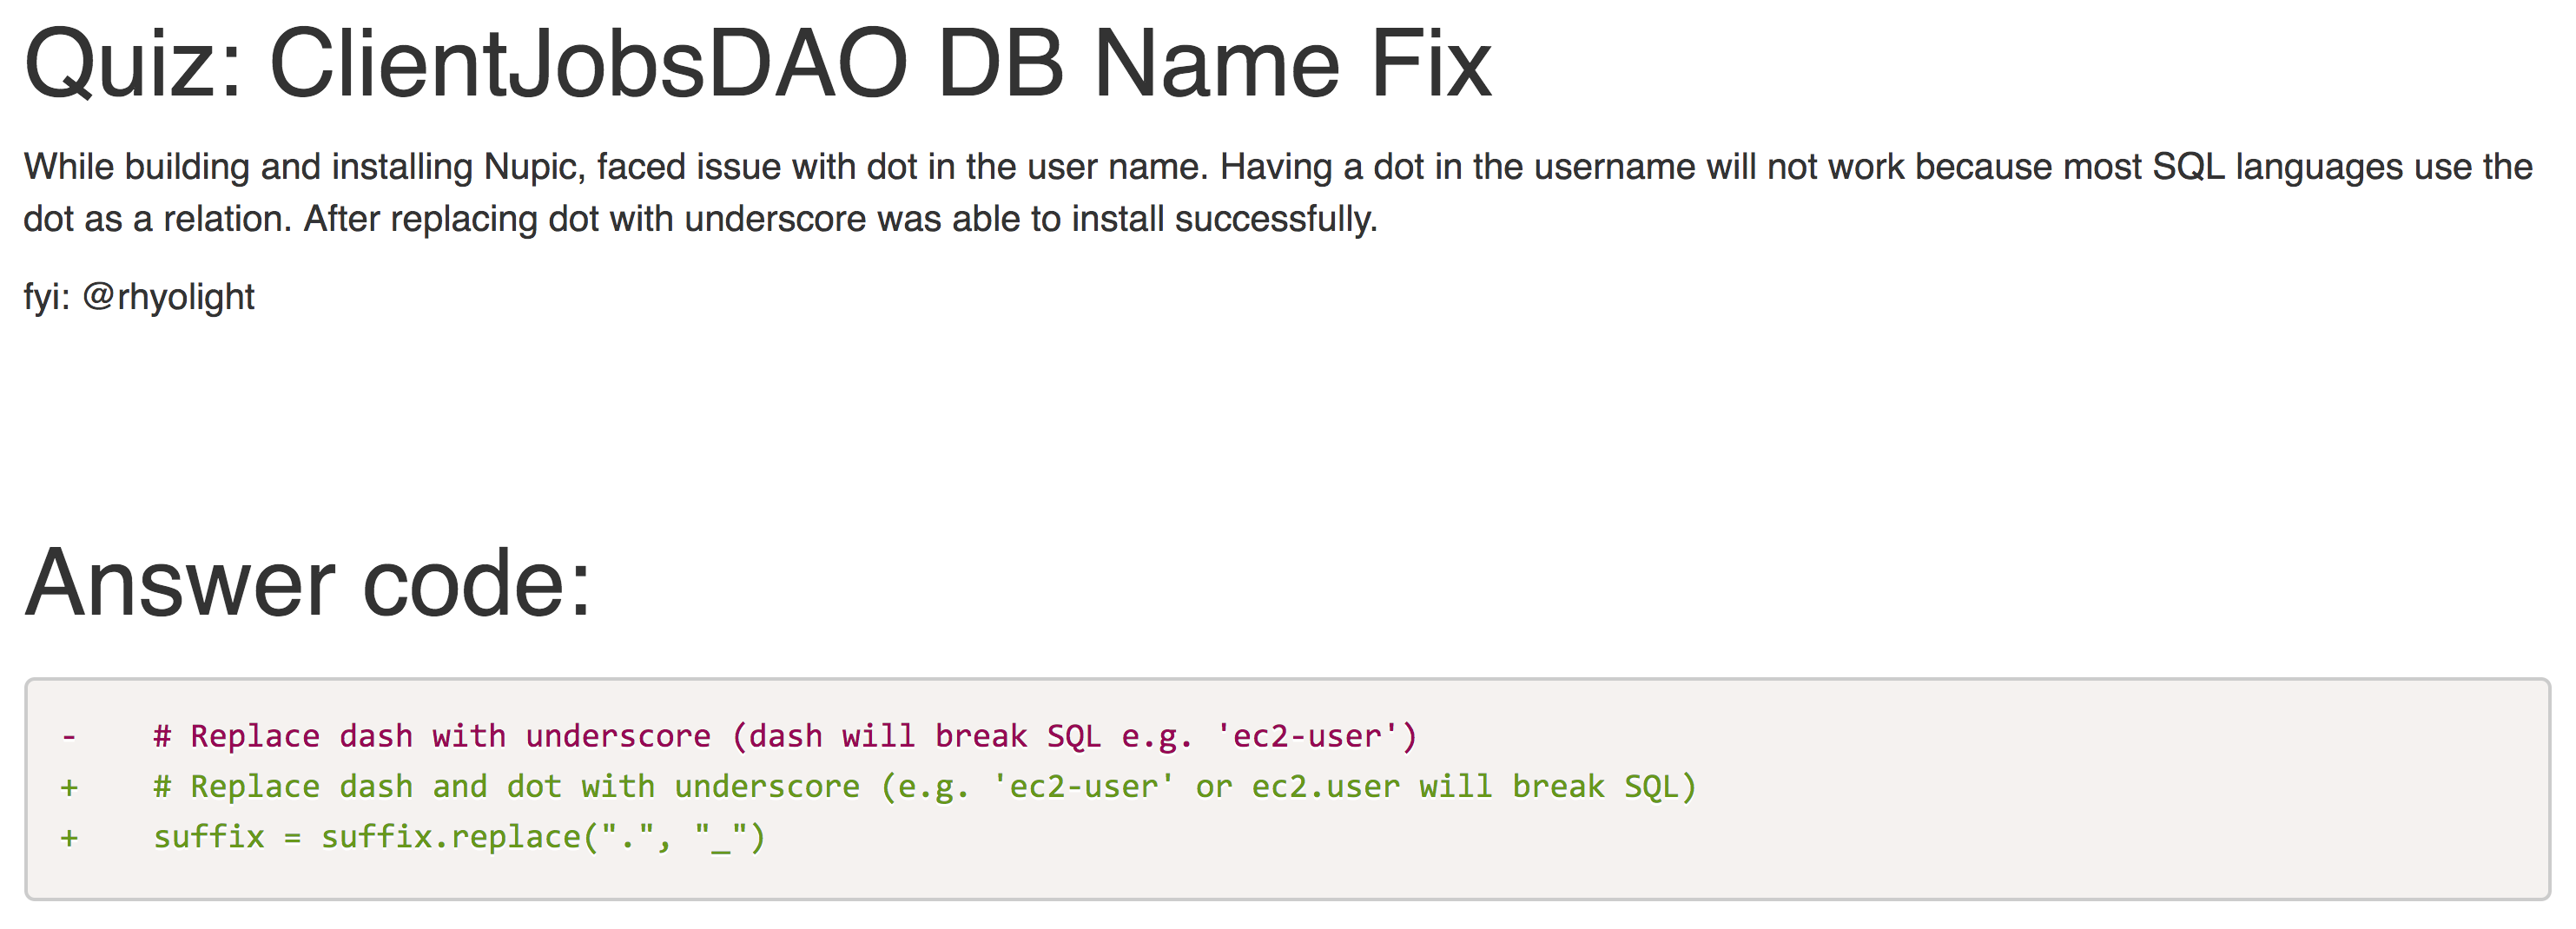
\includegraphics[width=0.95\columnwidth]{20190107-lab-study-experience-exercise.png}
  \caption{自分が経験した・見たことのあるバグの解決方法に関する演習問題の例.}
  \label{fig:lab-study-eg-experience}
  \vspace{-0.2cm}
\end{figure}


\subsection{ライブラリやAPIの使い方に関する演習問題}

実際のソフトウェア開発では,既に機能がパッケージとして実装されたライブラリを活用することで開発を効率的に進めている~\cite{Leveraging_API}.
図\ref{fig:lab-study-eg-lib}に示す演習問題の例は,Pythonのseaborn\footnote{\url{https://github.com/mwaskom/seaborn}}というデータの可視化に使用されるライブラリにおける,表のグリッド線の表示方法に関する問題である.
このように,RealCodeの演習問題を通じてライブラリを使用する上で発生しうる問題を学習できる可能性がある.

\begin{figure}[H]
\vspace{0.3cm}
	\centering
  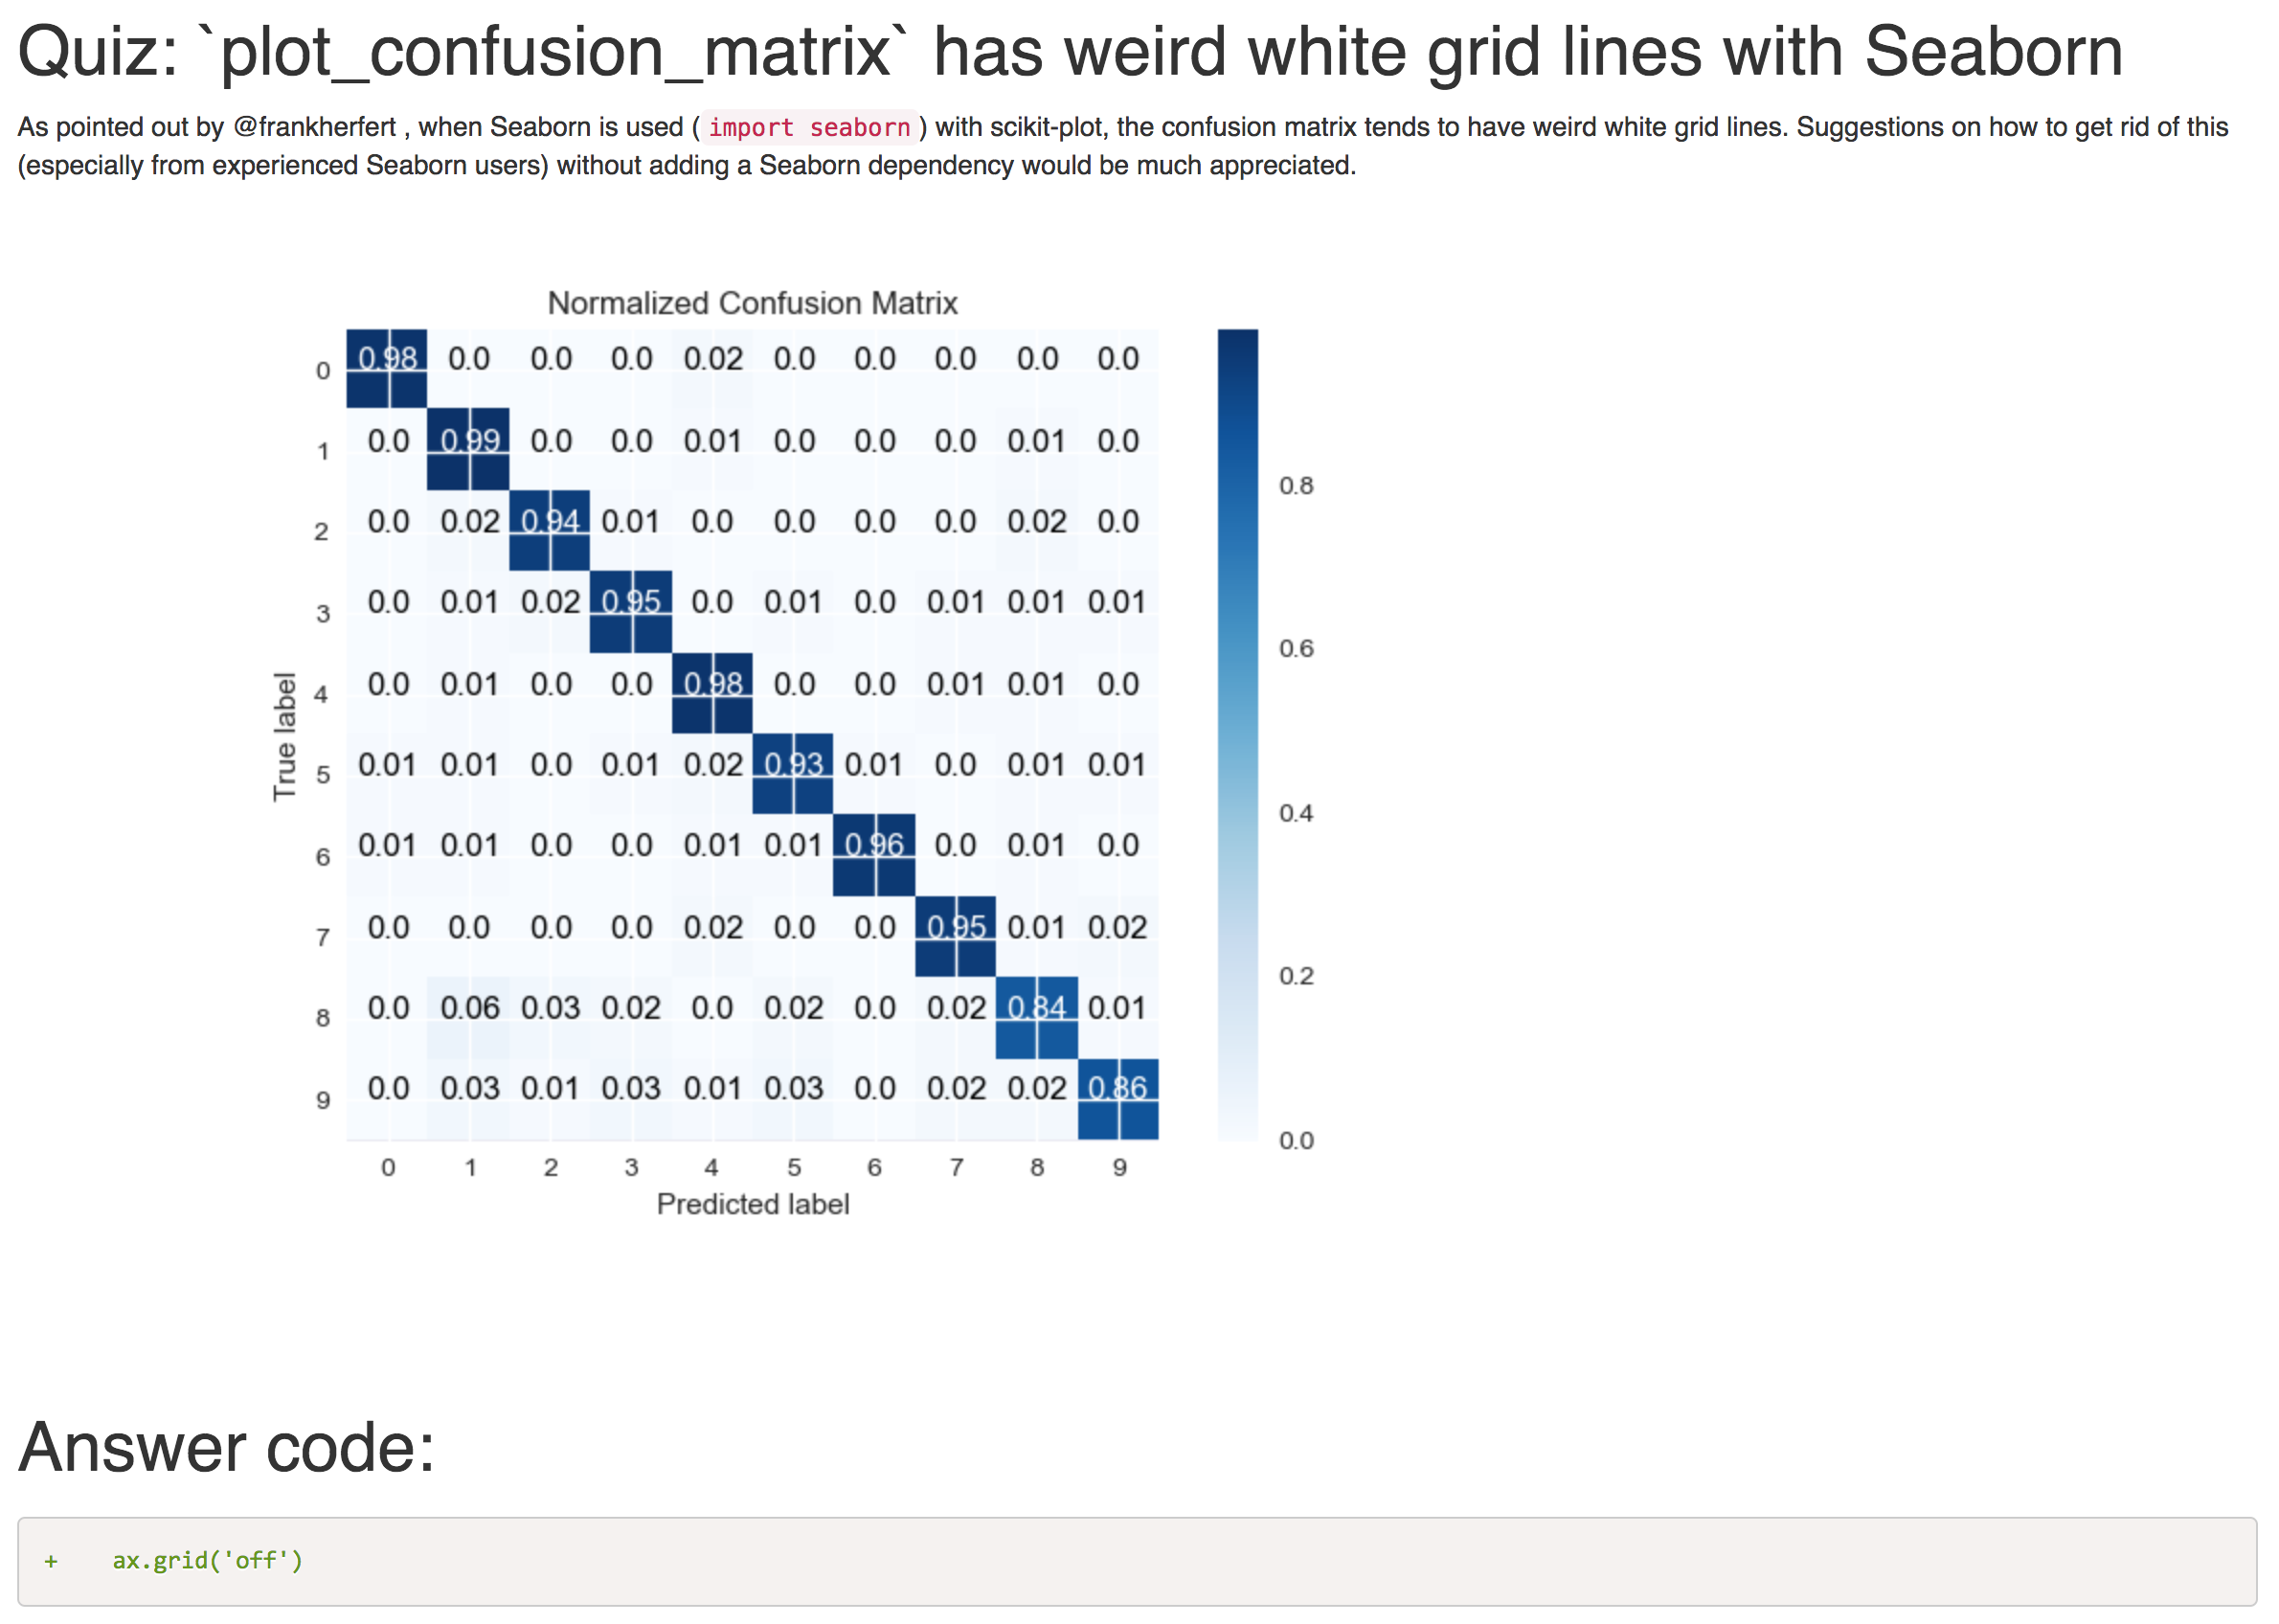
\includegraphics[width=1.0\columnwidth]{20190107-lab-study-lib-exercise.png}
  \caption{ライブラリやAPIの使い方に関する演習問題の例.}
  \label{fig:lab-study-eg-lib}
\end{figure}
